\documentclass[11pt]{article}
\usepackage{geometry}                % See geometry.pdf to learn the layout options. There are lots.
\geometry{letterpaper}                   % ... or a4paper or a5paper or ... 
%\geometry{landscape}                % Activate for for rotated page geometry
%\usepackage[parfill]{parskip}    % Activate to begin paragraphs with an empty line rather than an indent
\usepackage{graphicx}
\usepackage{amssymb}
\usepackage{epstopdf}

\usepackage{amsmath}
\usepackage{amssymb}

\usepackage{placeins}
\usepackage{harpoon}

\usepackage{longtable}

\usepackage{hyperref}
\hypersetup{
    colorlinks=true,
    linkcolor=blue,
%    filecolor=magenta,      
    urlcolor=blue,
}
 

\usepackage[square,numbers]{natbib}

\DeclareGraphicsRule{.tif}{png}{.png}{`convert #1 `dirname #1`/`basename #1 .tif`.png}

%\input{Macros.tex}
\title{HPS Note:  Beam Charge in the 2016 Data}
\author{Sebouh Paul}
\date{}                                           % Activate to display a given date or no date

\begin{document}
\maketitle

\section{Beam Blocker}
Due to the presence of the beam blocker in front of the Faraday cup in 2016, the calculation of the charge is more complicated than it was in 2015, in that the attenuation factor from the beam blocker is not known a priori.  Therefore, to determine the beam charge per run or per file, we need to use several pieces of information.  First, I had to calculate the offset to be subtracted from the Faraday cup readout, which I calculated using the beam trips.  Then, I calculated the ratio of the Faraday cup readout (with offset subtracted) to the measured current from the beam position monitor (BPM) 2C21A while the beam blocker is in place.  Next, i calculated the ratio of the Faraday cup measurement to the BPM measurement while the beam blocker was removed (during a 2 minute interval in run 7795).  The beam blocker attenuation factor was then given by:

\begin{equation}\label{eq:attenuation}
\textrm{attenuation factor} = \frac{\textrm{Faraday cup to BPM ratio (no beam blocker)}}{\textrm{Faraday cup to BPM ratio (no beam blocker)}}
\end{equation}

\section{Faraday Cup Offset}
I determined the value of the zero-point offset for the Faraday cup for each run using the value measured during the first beam-trip during the run.  If there was no beam trip during a run, i used the value from the previous run.  Specifically, i waited until the Faraday cup readout value dropped below a certain threshold (500 counts) remained below that threshold for 10 samples, and used the 10th sample as the offset.  

There was a significant variation in the value of the zero-point: the minimum value that I found was 12, and the maximum I found was 412.  However, these variations were on a much larger timescale than the duration of the run.  
Figure \ref{fig:zero_point} shows the measured zero-point of each of the runs in the preliminary golden run set.  

\begin{figure}[htbp] 
\begin{center}
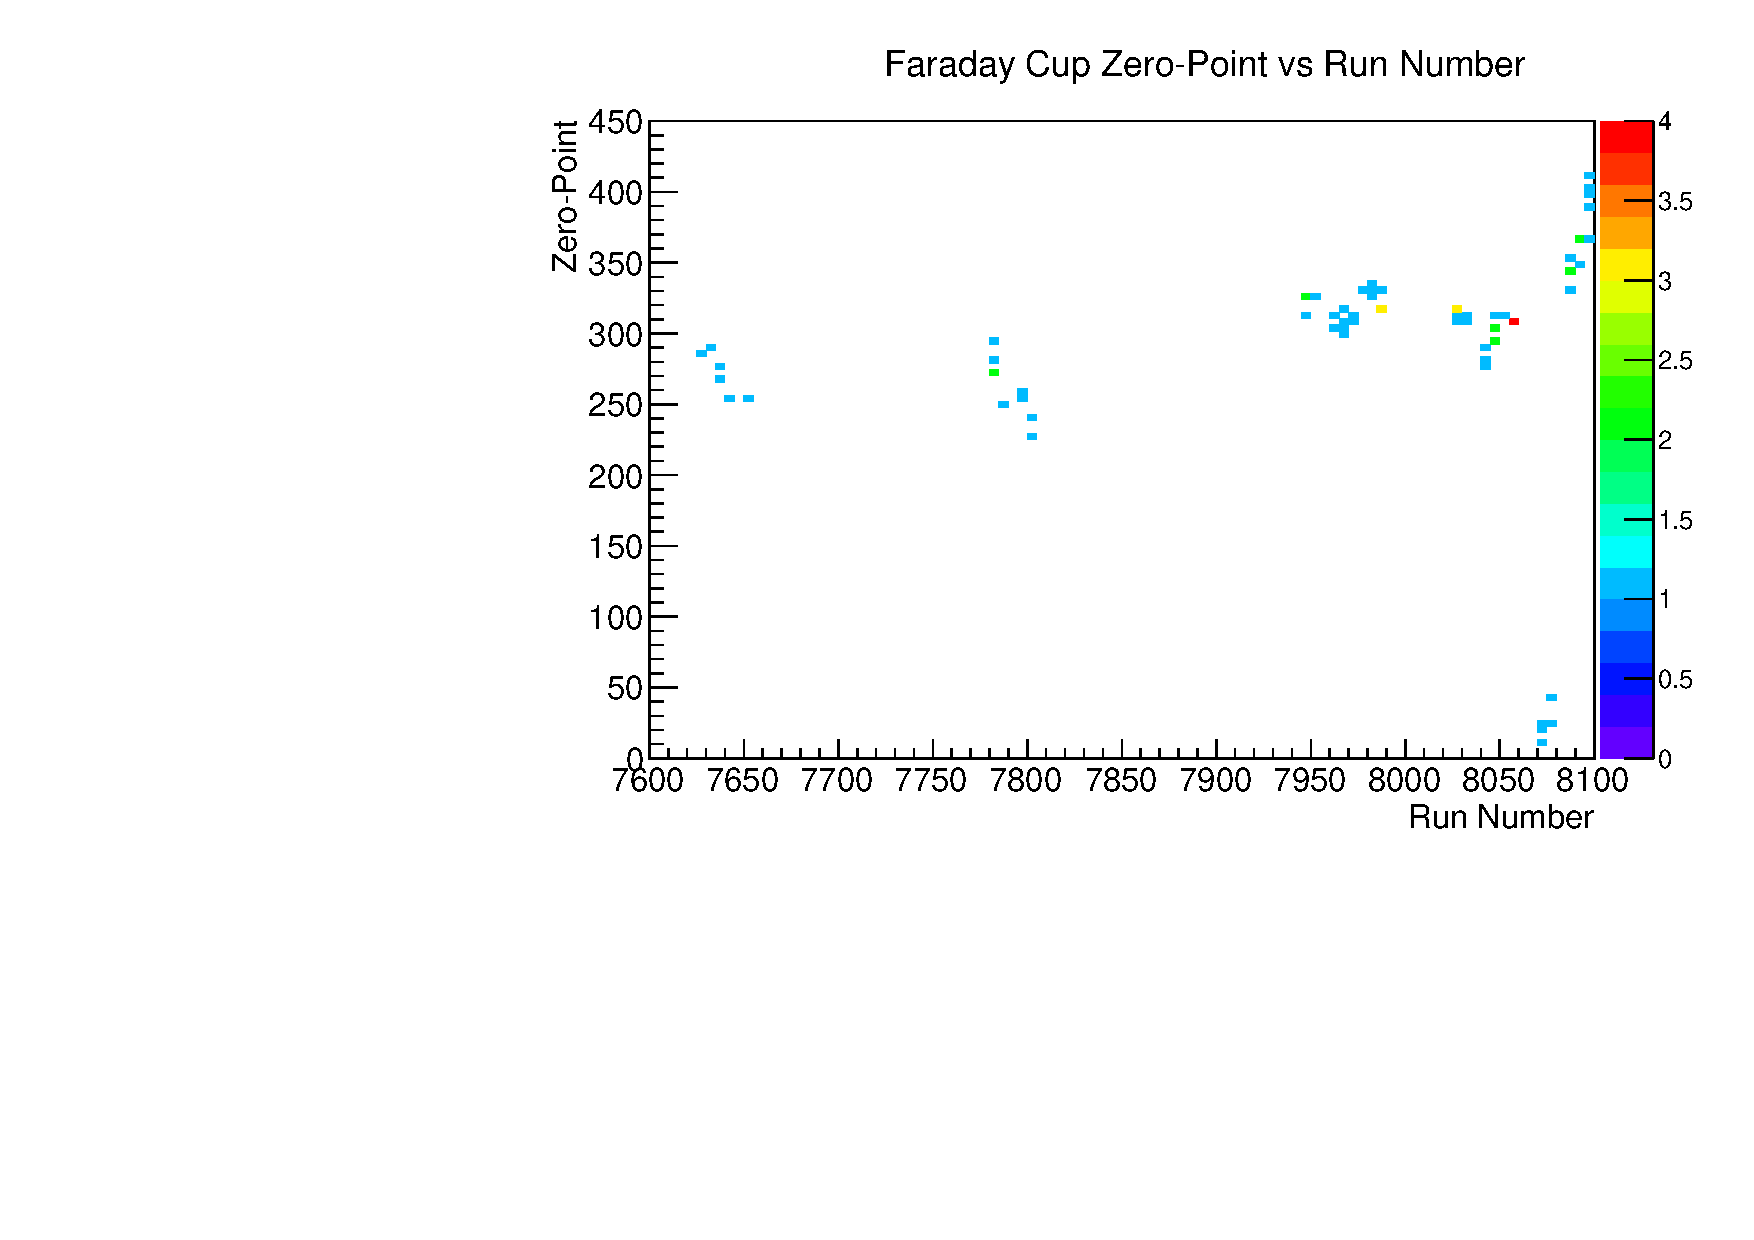
\includegraphics[width =  .9\textwidth]{figures/zeropoint.pdf}
\label{fig:zero_point}
\caption{Faraday Cup zeropoint offset, as measured during the beam trips.} 

\end{center}
\end{figure}



\section{Faraday Cup to BPM Ratio (with beam blocker)}

I also measured the ratio of the BPM readout to the faraday cup readout (with the offset subtracted).  I calculated the average value for this quantity for each of the runs.  In this calculation, i excluded samples that took place either during a beam trip or less than 15 seconds after the end of the beam trip.  

The ratio of the offset-subtracted faraday cup readout to the BPM measured current (in nA) remained approximately constant, with a mean of 14.48 and a standard deviation of 0.12 for the preliminary set of ``golden runs".  I excluded run 7795 in this calculation, because the beam blocker was removed for part of this run.
Figure \ref{fig:beam_blocker_ratio} shows the ratio between the Faraday cup measurement and the BPM measurement for many the preliminary golden run candidates.

\begin{figure}[htbp] 
\begin{center}
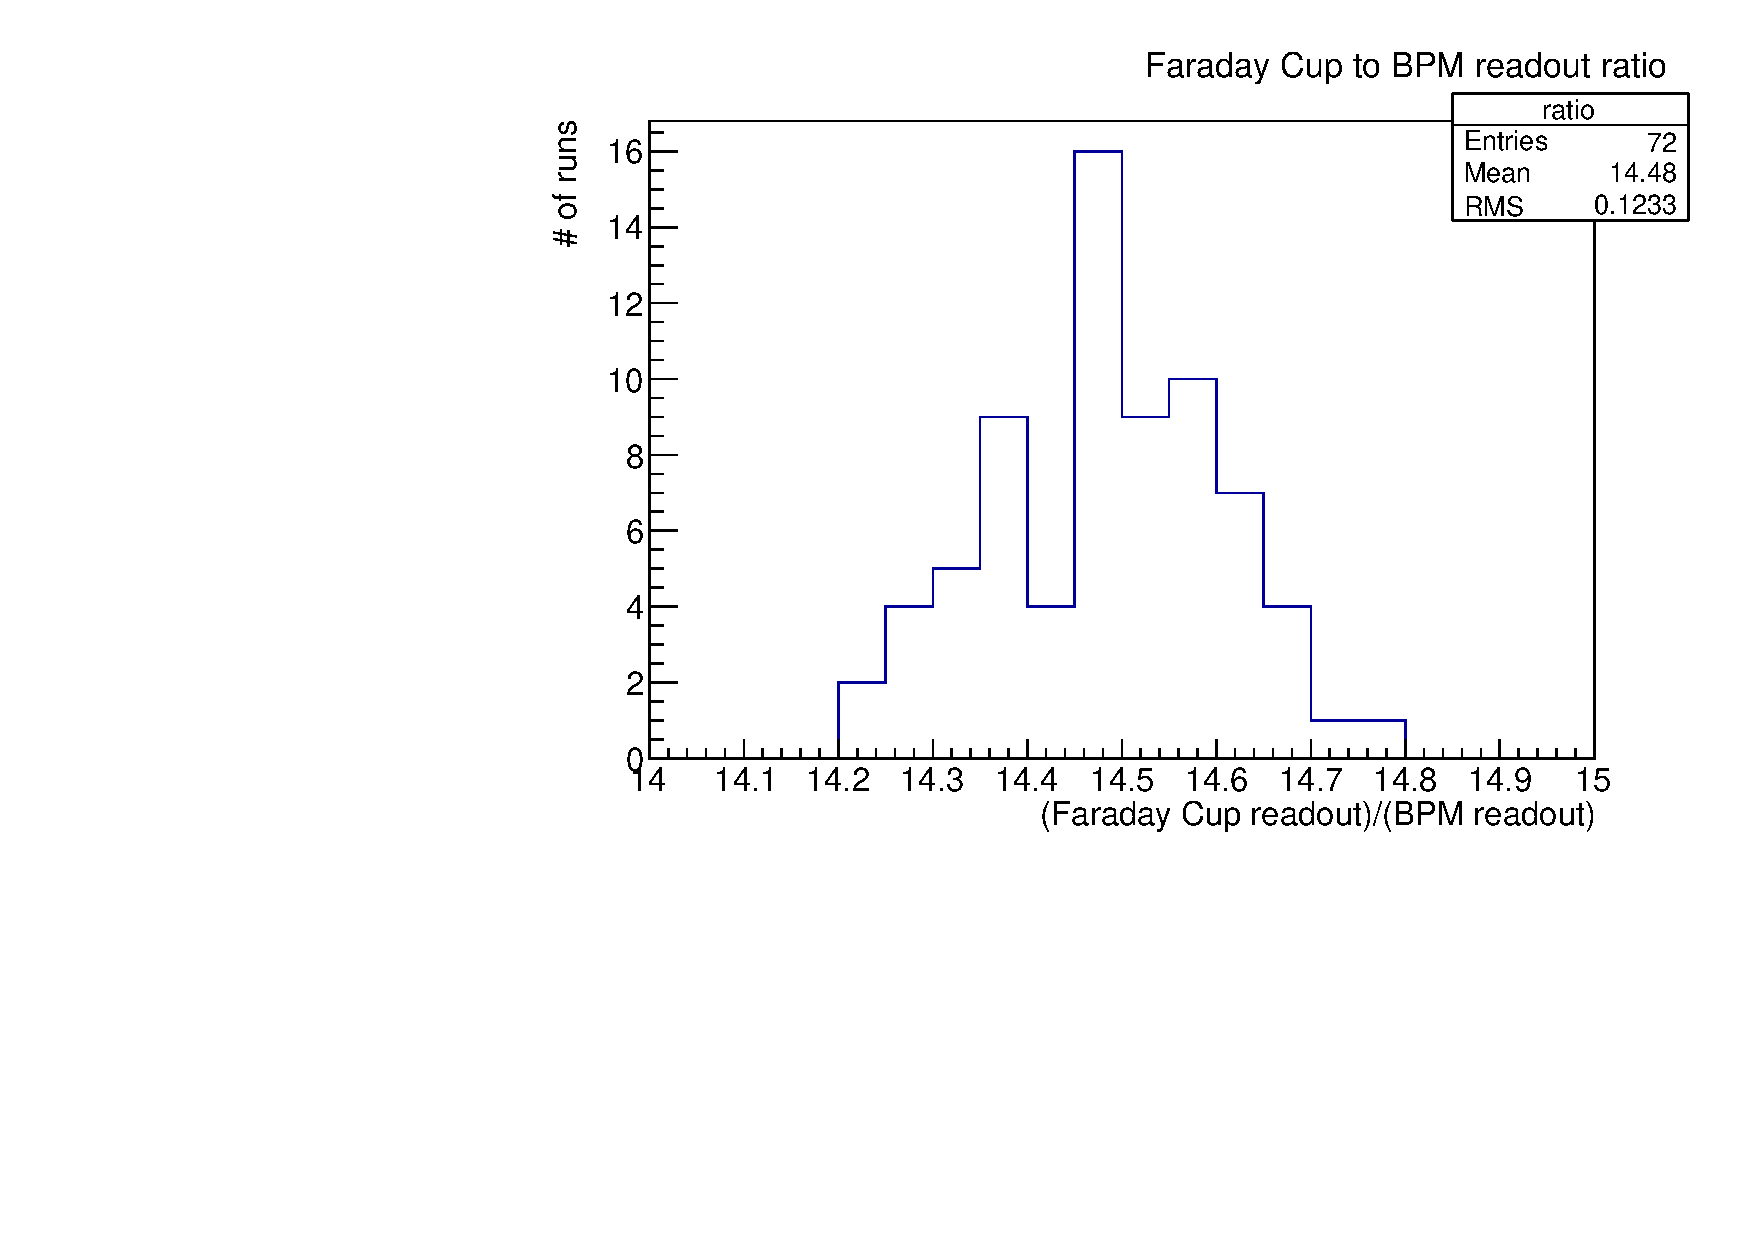
\includegraphics[width =  .9\textwidth]{figures/beam_blocker_ratio.pdf}
\label{fig:beam_blocker_ratio}
\caption{Ratio of the Faraday Cup readout to the BPM readout, plotted out per run.} 

\end{center}
\end{figure}


\section{Faraday Cup to BPM Ratio (without beam blocker)}

There was only a short interval (about 2 minutes) where the beam blocker was not in place during our entire run period, only about 1 minute of which had stable beam.  Dividing one of the samples of the Faraday cup readout (scalerS2B) during this time to the corresponding BPM measurement, the ratio of these two values is 897.5.

Figure \ref{fig:no_beam_blocker} shows the Faraday cup readout and the BPM readout during part of this interval while the beam was stable.

\begin{figure}[htbp] 
\begin{center}
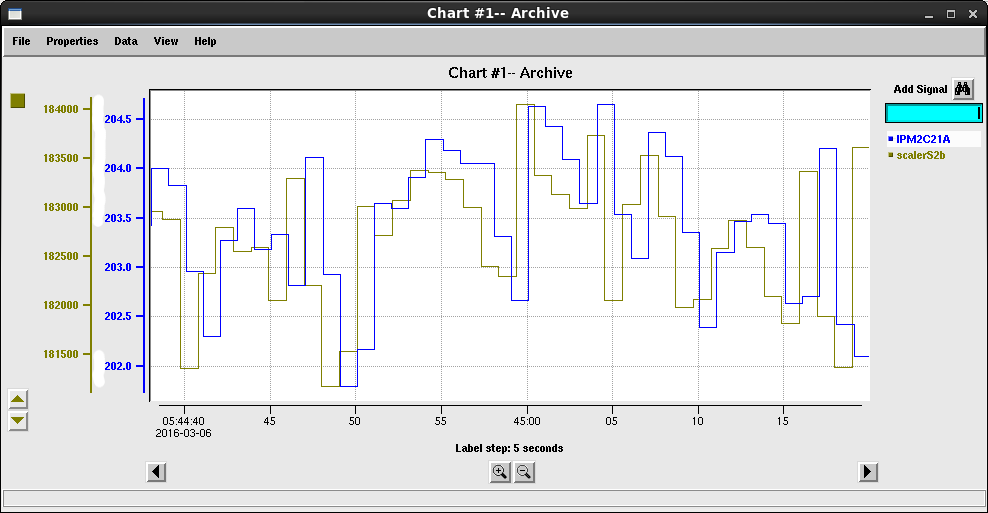
\includegraphics[width =  .9\textwidth]{figures/no_beam_blocker.png}
\label{fig:no_beam_blocker}
\caption{Faraday Cup and BPM readouts while the beam blocker was removed, as displayed in MyaViewer.} 

\end{center}
\end{figure}
  

\section{Conclusion}
By dividing the Faraday Cup to BPM ratio without the beam blocker by the same ratio with the beam blocker (see Equation \ref{eq:attenuation}), I determined the attenuation factor on the BPM to be 61.98.  Without the beam blocker, the conversion from the Faraday cup readout to the attenuation factor is 

\begin{equation}\label{eq:without_blocker}
\textrm{beam current} = \frac{\textrm{Faraday cup readout}-\textrm{offset}}{906.2} \textrm{nA}
\end{equation}

Therefore, to convert a Faraday cup reading \textit{with} the beam blocker to nA:

\begin{equation}\label{eq:with_blocker}
\textrm{beam current} = \frac{\textrm{Faraday cup readout}-\textrm{offset}}{906.2}*61.98 \textrm{nA}
\end{equation} 

After determining the parameters for this formula, I ran a modified version of Sho Uemura's SvtChargeIntegrator program, which calculate the beam charge per-run and per-file, with and also determines how much of this charge accumulated when the  SVT bias is on.   My modification was adding in the option to read in a text file which contains per-run values of the zeropoint offset and also the scaling factor between the Faraday cup measurement and the actual current.  I have placed the output of this program in the \href{https://docs.google.com/spreadsheets/d/1X_TfOQyQBv9Ja1IQ5LYImk0sd00eN-d4zzkCwn-CSUM/edit#gid=43855609}{\underline{2016 run spreadsheet}}, in the runsummary and filesummary sheets for the per-run and per-file beam charges respectively.  

There were several problems that we faced in the 2015 run that were not relevant in 2016.  For instance, we did not retract the SVT during beam trips, so it is not necessary to determine how much of the beam charge occurred while the SVT was at 0.5 mm is not relevant.  Secondly, we fixed the issue with the latency (which affected 2/6 trigger phases) prior to taking data in 2016.  Thirdly, we did not have errors in the headers of the files, since the bug that caused this was fixed.   Taking these things into consideration, I omitted the columns for beam charge "at nominal".   Additionally, I replaced the values of in the ``good beam charge" columns with the values in the  ``gated beam charge" columns, scaled by a factor of $1-f_{burst-mode}$, where $f_{burst-mode}$ is the fraction of the events affected by burst-mode noise (1.3\% in the 2016 data, as compared to 3.5\% in the 2015 dataset).  

Note: In run 7795, the beam blocker was removed during file 142 and was put back in place during file 149.  Therefore, the values in those rows of the file summary page are incorrect and should not be used.  I therefore included an extra row in the run summary sheet for run 7795 (titled "7795*") with the values from these files subtracted out.  

\end{document}